\documentclass[8pt]{report}
\usepackage{amsmath,amsfonts,amsthm} 

\usepackage{chngcntr}
\usepackage[parfill]{parskip}
\usepackage{graphicx} 
\usepackage{float}
\usepackage{epstopdf} 
\usepackage{subcaption}
\usepackage{enumitem}
\usepackage[colorlinks,urlcolor=blue]{hyperref}
\usepackage{listings}
\usepackage{pgfplots} 
\usepackage[a4paper, total={6in, 8.5in}, footskip=50pt]{geometry}
\usepackage{fancyhdr} 
\setlength{\parskip}{6pt}

\usepackage{tabto}


\usepackage{graphicx} 
\usepackage{float}

\usepackage[colorlinks,urlcolor=blue]{hyperref}
\usepackage{listings}
{geometry}
\usepackage{fancyhdr} 
\setlength{\parskip}{6pt}

\hypersetup{
    colorlinks,
    citecolor=black,
    filecolor=black,
    linkcolor=black,
    urlcolor=blue
} %Hyperlink setup for linking content pg and text
\pagestyle{fancy}

\begin{document}

%----------------------------------------------------------------------------------------
%	TITLE PAGE
%----------------------------------------------------------------------------------------

\begin{titlepage} % Suppresses displaying the page number on the title page and the subsequent page counts as page 1
	\newcommand{\HRule}{\rule{\linewidth}{0.5mm}} % Defines a new command for horizontal lines, change thickness here
	
	\center % Centre everything on the page
	
	%------------------------------------------------
	%	Headings
	%------------------------------------------------
	
	\textsc{\LARGE REPORT 1}\\[1 cm] % Main heading such as the name of your university/college
	\begin{figure}[h!]
\centering

\includegraphics[scale=1]{IITM.png}
\label{fig:boat}
\end{figure} 

	 	\textsc{\large Department Of Aerospace Engineering}\\[0.5cm] % Minor heading such as course title
	
	\textsc{\Large Indian Institute Of Technology, Madras}\\[0.5cm] % Major heading such as course name
	
	%------------------------------------------------
	%	Title
	%------------------------------------------------
		\HRule\\[0.4cm]
	
	{\huge\bfseries DESIGN OF UAV}\\[0.4cm] % Title of your document
	{\large\bfseries UDAAN}\\
	\HRule\\[1.5cm]
	
	%------------------------------------------------
	%	Author(s)
	%------------------------------------------------
	
	
\begin{table}[h!]
 \begin{center}
 \begin{tabular}{|c| c |c |c|} 
 \hline
 NAME & ROLL.NO & JOB & PERCENTAGE \\ [0.5ex] 
 \hline
 Suyash Singh & AE17M009 & Report Writing & 20 \\ 
 \hline
  Krishna Kumar & AE17M017  & Report Writing & 20 \\
 \hline
 Ankit Kukadia & AE17M018  & Report Writing & 20 \\
 \hline
 Akhil Sangaonkar & AE17M023 & Report Writing & 20 \\ 
 \hline
 Vaibhav Khandelwal & AE17M032 & Report Writing & 20 \\ 
 \hline
 Sumit Sharma & AE17M038 & Report Writing & 20 \\ 
 \hline
\end{tabular}
\end{center}

\end{table}
	
	% If you don't want a supervisor, uncomment the two lines below and comment the code above
	%{\large\textit{Author}}\\
	%John \textsc{Smith} % Your name
	
	%------------------------------------------------
	%	Date
	%------------------------------------------------
	
	\vfill\vfill\vfill % Position the date 3/4 down the remaining page
	
	{\large\today} % Date, change the \today to a set date if you want to be precise
	
	%------------------------------------------------
	%	Logo
	%------------------------------------------------
	
	%\vfill\vfill
	%\includegraphics[width=0.2\textwidth]{placeholder.jpg}\\[1cm] % Include a department/university logo - this will require the graphicx package
	 
	%----------------------------------------------------------------------------------------
	
	\vfill % Push the date up 1/4 of the remaining page
	
\end{titlepage}

%----------------------------------------------------------------------------------------

\end{document}


\hypersetup{
    colorlinks,
    citecolor=black,
    filecolor=black,
    linkcolor=black,
    urlcolor=blue
} %Hyperlink setup for linking content pg and text
\pagestyle{fancy}
\fancyhf{}
\rhead{{\small \leftmark}}
\cfoot{\thepage}
\renewcommand{\footrulewidth}{.5pt} 
\renewcommand{\headrulewidth}{.5pt}
\renewcommand{\baselinestretch}{1.3}

\begin{document}
\tableofcontents{}
\let\cleardoublepage\relax
\thispagestyle{empty}

\listoffigures{}
\addcontentsline{toc}{section}{\numberline{}List of figures}
\pagenumbering{roman}
\setcounter{page}{1}
\listoftables{}
\addcontentsline{toc}{section}{\numberline{}List of Tables}
\pagebreak
\pagenumbering{arabic}
\chapter{First Weight Estimation}
\section{Introduction}
To develop UDAAN - a lightweight, energy efficient, inflatable drone capable of vertical Take off, Stand By and Landing, which can deliver payloads and is self rechargeable.
Drones allows for a wide variety of missions, however with the weight of the sensors increasing, the drones able to carry such payloads are cumbersome and difficult to transport.That is why we are trying to develop India's first inflatable drone.The drone has inflatable structure, is at the same time will be easy to transport and rugged because of the flexible structure. Moreover, the drone would be waterproof and can land and take-off on water surface because of compressed Helium gas used in the inflatable structure. 


\section{Novelty Features}

\subsection{Fast}

The UDAAN will unfold in a few seconds and can be operated by a single person.

\subsection{Compact}

The UDAAN will be easily transportable thanks to its compact and foldable inflatable structure

\begin{figure}[h!]
\centering
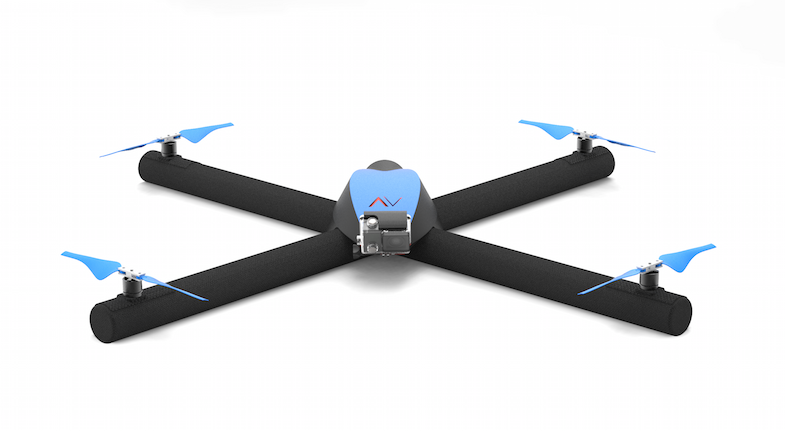
\includegraphics[width=.8\textwidth]{drone.png} 
\caption{\label{fig:drone}Inflatable drone}
\end{figure}

\subsection{Amphibious}

The UDAAN is waterproof, therefore deployable under heavy rain or even on water.

\subsection{Payload and Surveillance}

UDAAN is capable of carrying a Payload and hence can be utilised for delivery of items via e-commerce channel.


\subsection{Self Rechargeable}

UDAAN would be equipped with self rechargeable capabilities.We are trying to develop and incorporate a mechanism to recharge the battery using renewable energy sources. 

.


\clearpage
\section{Mission Profile} .

\begin{figure}[h!]
\centering
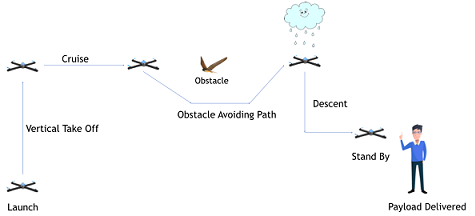
\includegraphics[width=1.1\textwidth]{mission_profile.png} 
\caption{\label{fig:mission_profile}Mission Profile}
\end{figure}


\section{Estimated Data}

\subsection{Dimensions}

Available Payload : Camera, Parcel

Folded : 300x300x150 mm

Unfolded : 800x800x150 mm

Endurance : up to 60 min

\subsection{Common Characteristics}

Waterproof

Wind resistance : 37 kmph

Unfolding time : ‹60s

Folding time : ‹60s

\subsection{Weight Estimate}
The approximated weight of the UDAAN will be 300-500gm, which will be depend upon material used and the battery required.

\bibliographystyle{alpha}
\bibliography{sample}
\chapter{Second Weight Estimation}

\section{Weight Estimate}
\begin{itemize}
\item Propeller = 30 grams

\item Motor = 4 * 23 = 92 grams

\item Flight Control Board = 60 grams

\item Electronic speed controller = 4 * 100 = 400 grams

\item Base weight = 200 grams

\item Bolts = 20 grams

\item Locking nuts = 20 grams

\item Wires = 30 grams

\item Camera weight = 100 grams

\item Battery = 160 grams (2200mah)



\item Total weight = 1112 grams

\end{itemize}
\section{Thrust Calculation}

\begin{itemize}

\item Estimated Weight of drone = 1112 grams

\item Thrust/Weight = 2

\item Headspace given for thrust = 20 \%

\item Net thrust required = 2.4 * 1112 grams = 2669 grams

\item Net thrust required per motor = 670 grams

\item Specification of propeller:
\begin{enumerate}
\item Diameter = 8 inches
\item pitch = 4 inches
\end{enumerate}
\end{itemize}

\subsection{Motor Specification}

Motor: Avionic M2226/18 KV2570 MICRO brushless motor

KV (rpm/v): 2570

Power: 80W

Winds: 18

Resistance: 327 mOhm

Idle current: 0.8 A

Weight: 23 gms



\subsection{Formula used for thrust calculation}

\begin{figure}[h!]
\centering

%\includegraphics[scale=0.8]{thrustformula.jpeg}
\label{fig:boat}
\end{figure}


\begin{figure}[h!]
\centering

%\includegraphics[scale=0.8]{Capture.png}
\caption{fig.thrust v/s graph}
\label{fig:boat}
\end{figure}

\subsection{Battery Specification}

Minimum Capacity: 2200mAh

Configuration: 3S1P / 11.1v / 3Cell

Constant Discharge: 25C

Peak Discharge (10sec): 35C
\section{Procedure}
\begin{itemize}

\item Decide appropriate dimension of propeller.
\item Choose suitable RPM of motor.
\item Get the required static thrust from the table.
\item Iterate the dimensions until you get the required thrust which is 672 g of thrust.
\item After fixing the dimension and RPM of motor, find suitable LiPo battery
\item RPM = KV * Battery voltage
RPM = 2570 * 11.1 = 28500
\item This is the RPM of motor without propeller.After using propeller RPM reduces by 2.5 times approximately.
\item Net RPM = 11410 (estimated)
\item After finalizing the battery, fix the Electronic speed controller.
\end{itemize}
  
\section{Conclusion} 
The weight of the inflatable drone is estimated to be around 1112g.The estimated static thrust produced is 6.636 N.In the next phase, after performing successive iterations we will finalize the weight of the drone and perform dynamic thrust calculations.

\section{References}
  
\begin{enumerate}

\item http://www.rcbazaar.com/product.aspx?productid=2400


\item http://www.3drcparts.com/zippy-2200mah-11-1v-3s-25-35c-light-weight-lipo-battery/


\item https://www.flitetest.com/articles/propeller-static-dynamic-thrust-calculation
\end{enumerate}
\end{document}